%------------------------------------------
% Szakdolgozat
% 
% 
% Varga Roland
%
% Konzulens: Magyar László
%------------------------------------------

\documentclass[12pt,a4paper,twoside]{article}
\usepackage{dissert}
% \renewcommand{\familydefault}{ptm}

\begin{document}
\frontmatter
\author{Varga Roland}
\title{Ember és robot interakciójának demonstrációja\\
		Sakkozó iiwa robotkar}
%--Szennycímoldal-----------------------------------------
\newpage\thispagestyle{empty}
\begin{center}
     VARGA ROLAND\\
     SZAKDOLGOZAT
\end{center}
%--Sorozatcímoldal----------------------------------------
%\newpage\null\thispagestyle{empty}
\newpage\thispagestyle{empty}
\begin{center}
     BUDAPESTI MŰSZAKI ÉS GAZDASÁGTUDOMÁNYI EGYETEM\\
     GÉPÉSZMÉRNÖKI KAR\\
     MECHATRONIKA, OPTIKA ÉS GÉPÉSZETI INFORMATIKA TANSZÉK\\[1ex]
     \resizebox{2.5cm}{!}{
          
\includegraphics{figures/mogi.png}
     }\\[1ex]
     SZAKDOLGOZATOK
\end{center}
%--Címoldal-----------------------------------------------
%\newpage\null\thispagestyle{empty}
\newpage\thispagestyle{empty}
\begin{titlepage} %environment for unique titlepage design
\centering
\resizebox{4.5cm}{!}{
  
\includegraphics{figures/bme}
}\\[1ex]
{\bf BUDAPESTI MŰSZAKI ÉS GAZDASÁGTUDOMÁNYI EGYETEM}\\
{\bf GÉPÉSZMÉRNÖKI KAR}\\
{\bf MECHATRONIKA, OPTIKA ÉS GÉPÉSZETI INFORMATIKA TANSZÉK}\\[3cm]

{\LARGE \scshape Varga Roland}\\[2ex]
{\Large SZAKDOLGOZAT}\\[2ex]
{\Large \bf Ember és robot kooperációjának demonstrálása\\
		Sakkozó iiwa robotkar segítségével}\\[2ex]
{\itshape Demonstrating human-robot collaboration\\
				With chess-playing iiwa robotic arm}\\[5cm]

\begin{tabularx}{\textwidth}{XXXX}
Konzulens: & Témavezető: \\
\hspace{0.75cm} \itshape Magyar László & \hspace{0.75cm} \itshape Dr. Czmerk András \\
\hspace{0.75cm} tesztmérnök & \hspace{0.75cm} egyetemi adjunktus \\
\end{tabularx}\\[4cm]

{\Large Budapest, 2018}
\end{titlepage}

%--Záradék és nyilatkozatok-------------------------------
%%--Copyright oldal----------------------------------------
\newpage\null\thispagestyle{empty}
\newpage\thispagestyle{empty}
Szerzői jog \textcopyright ~Knyihár Gábor, 2018.\\[2cm]

\begin{center}
    \bf ZÁRADÉK
\end{center}


{\bf Ez a szakdolgozat elzártan kezelendő és őrzendő, a hozzáférése a vonatkozó szabályok szerint korlátozott, a dolgozat tartalmát csak az arra feljogosí-tott személyek ismerhetik.}

{\bf A korlátozott hozzáférés időtartamának lejártáig az arra feljogosítottakon kívül csak a korlátozást kérelmező személy vagy gazdálkodó szervezet írásos engedélyéjével rendelkező személy nyerhet betekintést a dolgozat tartalmába.}\\[0.5cm]

{\bf A hozzáférés korlátozása és a zárt kezelés 2023. év december hónap 
31. napján ér véget.}

%--Feladatkiírás lapja------------------------------------
\newpage\null\thispagestyle{empty}
\newpage\thispagestyle{empty}

%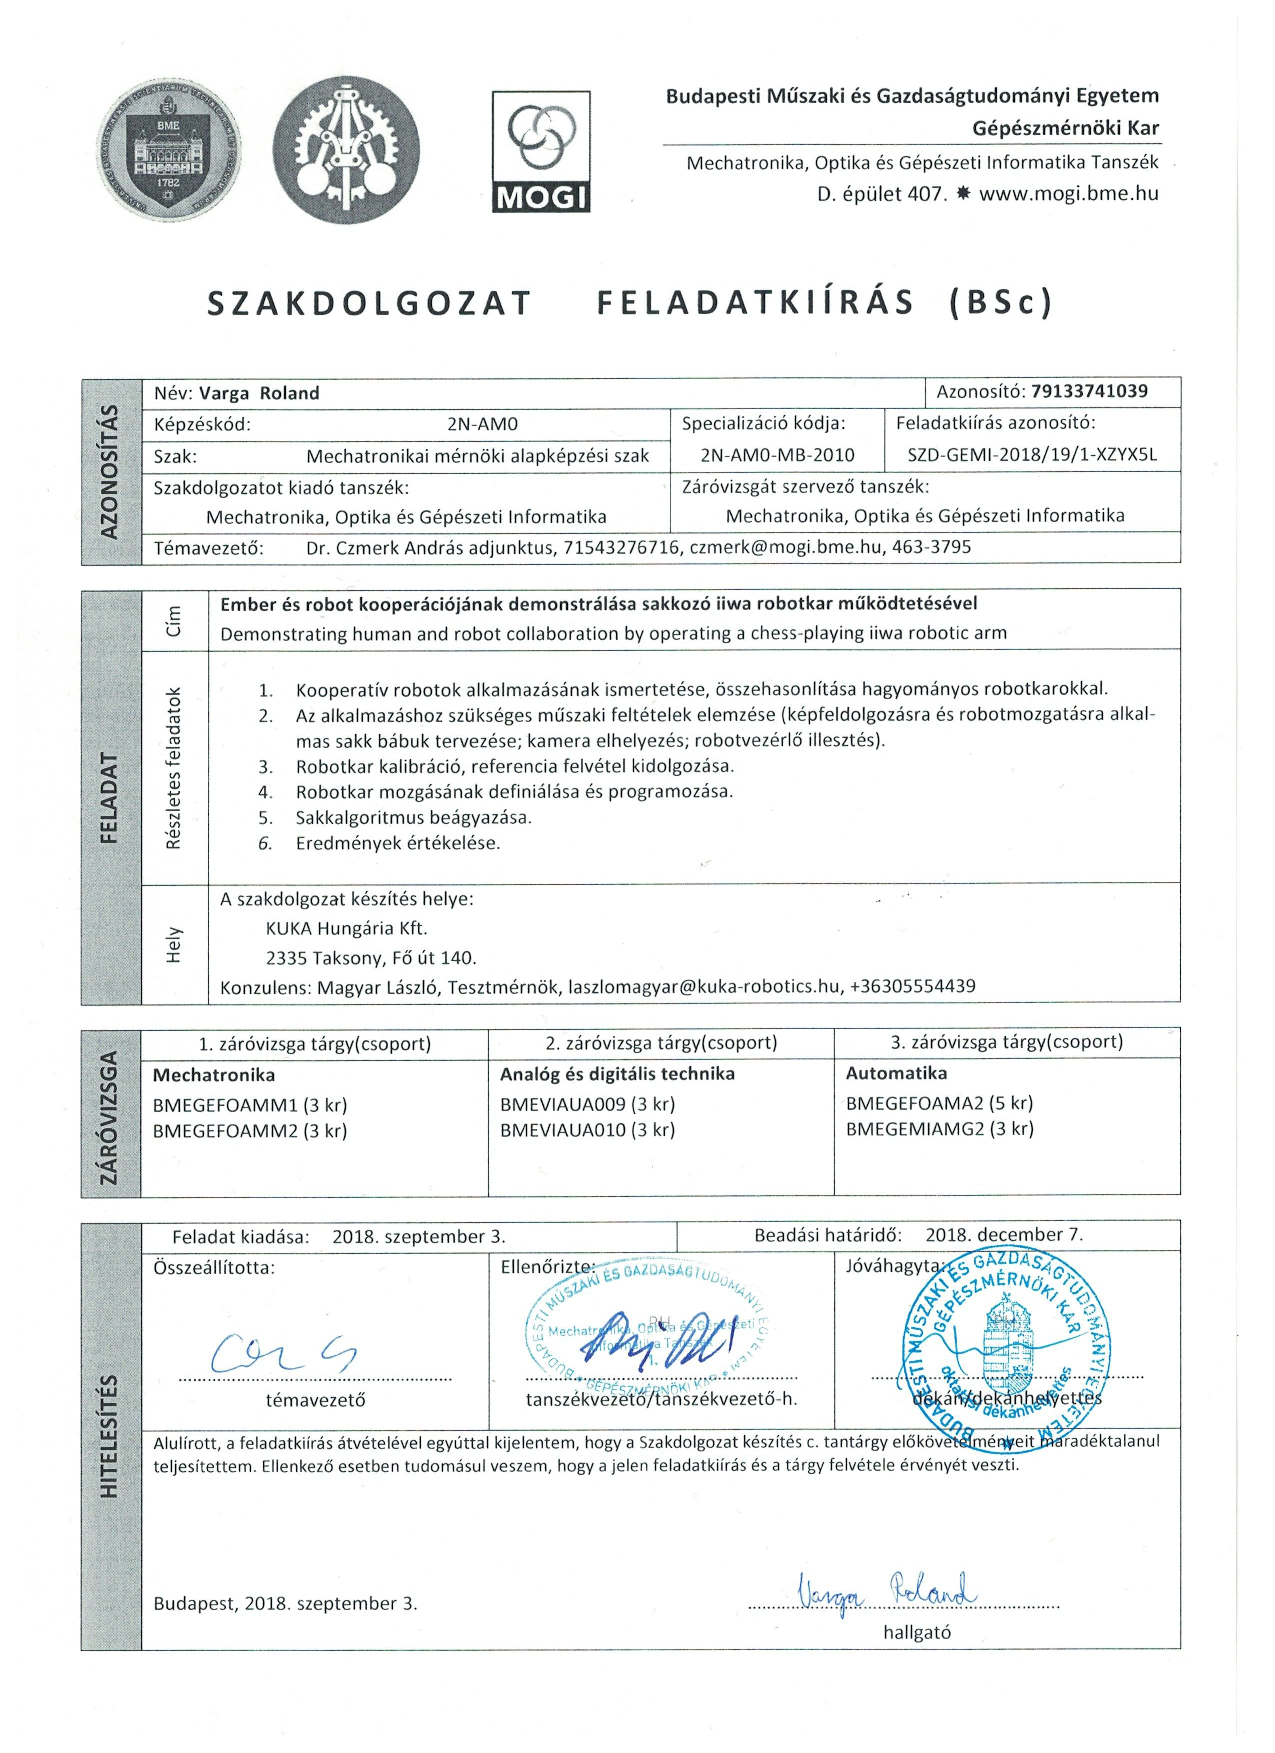
\includepdf[pages=-, offset=75 -75]{Figures/feladatkiiras.pdf}

%--Nyilatkozatok------------------------------------------
\newpage\null\thispagestyle{empty}
\newpage\thispagestyle{plain}
\begin{center}
    \Large \MakeUppercase{Nyilatkozatok}
\end{center}

{\centering \itshape Beadhatósági nyilatkozat \par}
A jelen szakdolgozat az üzem által elvárt szakmai színvonalnak mind tartalmilag, mind formailag megfelel, beadható.

Kelt, 

{\hspace{0.4\textwidth} Az üzem részéről:}\\[1cm]

{\hspace{0.6\textwidth} \itshape üzemi konzulens}\\[0.1cm]

{\centering \itshape Elfogadási nyilatkozat \par}
Ezen szakdolgozat a Budapesti Műszaki és Gazdaságtudományi Egyetem Gépészmérnöki Kara által a Diplomatervezési és Szakdolgozat feladatokra előírt valamennyi tartalmi és formai követelménynek, továbbá a feladatkiírásban előírtaknak maradéktalanul eleget tesz. E szakdolgozatot a nyilvános bírálatra és nyilvános előadásra alkalmasnak tartom. 

A beadás időpontja: \\[1cm]

{\hspace{0.62\textwidth} \itshape témavezető}\\[0.1cm]

{\centering \itshape Nyilatkozat önálló munkáról \par}
Alulírott, Varga Roland (XZYX5L), a Budapesti Műszaki és Gazdaságtudományi Egyetem hallgatója, büntetőjogi és fegyelmi felelősségem tudatában kijelentem és sajátkezű aláírásommal igazolom, hogy ezt a szakdolgozatot meg nem engedett segítség nélkül, saját magam készítettem, és dolgozatomban csak a megadott forrásokat használtam fel. Minden olyan részt, melyet szó szerint vagy azonos értelemben, de átfogalmazva más forrásból átvettem, egyértelműen, a hatályos előírásoknak megfelelően, a forrás megadásával megjelöltem.

{Budapest, 2018 ......................}\\[1cm]

{\hspace{0.6\textwidth} \itshape szigorló hallgató}

%--Tartalomjegyzék----------------------------------------
\newpage\null\thispagestyle{empty}
\newpage\thispagestyle{plain}
\tableofcontents

%--Előszó-------------------------------------------------
%\documentclass[../documentation.tex]{subfiles}
 
\begin{document}
\section*{Előszó}
Napjainkban egyre növekszik az igény arra, hogy a robotok az emberekkel kapcsolatba léphessenek, ne legyenek kerítésekkel elválasztva. Ilyen módon sokkal inkább ki tudják segíteni az embert, egyfajta technikai asszisztens szerepet láthatnak el. Olyan munkákat képesek elvégezni, amely az ember számára fárasztó, monoton vagy veszélyes lehet. 

A különféle robotokkal már nem csak ipari környezetben, hanem akár a gyógyászat területén is találkozhatunk. Ilyen robotok képesek például rehabilitációs tornákkal segíteni a betegeknek. Az ilyen mértékű együttműködésre tervezett robotok kialakításánál fontos szempont, hogy az ember biztonságban érezze magát mellettük. Ha egy robot tud vigyázni a körülötte lévőkre, mozgása gördülékeny, kiszámítható és jól alkalmazkodó, akkor sokkal könnyebb a bizalmat megadni neki.

A szakdolgozat célja az ember és a robot finom együttműködését bemutató robotalkalmazás kidolgozása. Ez egy társasjáték formájában valósul meg: lehetőség nyílik egy ipari robot ellen egy sakkjátszma lejátszására.


\end{document}
%--Jelölések jegyzéke-------------------------------------
\newpage\null\thispagestyle{empty}
\newpage\thispagestyle{plain}
\section*{Jelölések jegyzéke}

A táblázatban a többször előforduló jelölések magyar és angol nyelvű elnevezése, valamint a fizikai mennyiségek esetén annak mértékegysége található. Az egyes mennyiségek jelölése – ahol lehetséges – megegyezik hazai és a nemzetközi szak-irodalomban elfogadott jelölésekkel. A ritkán alkalmazott jelölések magyarázata első előfordulási helyüknél található.
%--Footer-------------------------------------------------
\newpage\null\thispagestyle{empty}
\newpage\thispagestyle{fancy}
%\include{boschfoot}

\mainmatter

%--Bevezetés----------------------------------------------
\section{Kooperatív robotkarok alkalmazása}


%--Irodalomkutatás----------------------------------------
%\documentclass[../documentation.tex]{subfiles}
 
\begin{document}

\section{Irodalomkutatás}
\subsection{Ipar 4.0 eredete}
Az Ipar 4.0 koncepcióját Németországban dolgozták ki, ahol világszinten kiemelkedő a termelési iparág, illetve világvezető a gyártó eszközök területén. Az Ipar 4.0 a német kormány stratégiai kezdeményezése volt, mely nagy mértékben támogatta az ipari szektor fejlesztését. Ilyen értélemben az Ipar 4.0-ra tekinthetünk egy olyan mozgalomként, amelynek célja megőrizni Németország befolyását a gépiparban és az autógyártás területén.\cite{industry40}

Az alap koncepciót először a Hanover Fair-en\footnote{A hannoveri a világy egyik legnagyobb kereskedelmi bemutatója. Körülbelül 6500 kiállító és 250.000 látogató vesz részt ezen a rendezvényen.} prezentálták 2011-ben. A bemutató óta az Ipar 4.0 Németország vezető témája a kutatások területén, egyetemi és ipari környezetekben különféle eseményeken. A fő irányvonal az új technológiákban és koncepciókban rejlő potenciál kihasználása felé mutat, ilyen területek:
\begin{itemize}
	\item az IoT (\foreignlanguage{british}{Internet of Things}\footnote{A Dolgok internete fizikai eszközökből, járművekből, otthoni felszerelésekből és további elektronikát, szoftvert, szenzorokat, aktuátorokat tartalmazó tételekből álló hálózat, amelyek képesek egymással kapcsolatba lépni, adatot fogadni és küldeni.}) elérhetősége és kihasználása,
	\item a technológiai és gazdasági folyamatok integrációja cégen belül,
	\item a valóság virtuális leképezése,
	\item `okos' gyárak beleértve az `okos' gyártást és termékeket.
\end{itemize}

\subsection{Előnyei}
Amellett hogy a digitalizáció és az új technológiák természetes következménye, az Ipar 4.0 megjelenése szintén kapcsolatban áll azzal a ténnyel, hogy a gyártásban a profit nővelésére irányuló kezdeményezések, lehetőségek nagy része kiaknázásra került, új megoldásokat kellett keresni. A gyártási költségek csökkentek a Just-In-Time (röviden JIT) termelés bevezetésével, a lean elveinek alkalmazásával és a gyárak olyan helyre telepítésével, ahol a munkaerő lényegesen olcsóbb. Ha az előállítási költségek minimalizálása a célunk, az Ipar 4.0 egy ígéretes megoldásnak tűnik. Számos forrás alapján az Ipar 4.0 alkalmazása csökkentheti\cite{industryresults}:
\begin{itemize}
	\item a gyártás költségét 10-30\%-kal,
	\item a logisztikával kapcsolatos kiadásokat 10-30\%-kal,
	\item a minőségmenedzsmenthez köthető költségeket 10-20\%-kal.
\end{itemize}

Ezeken kívűl a koncepció alkalmazásának számos egyéb előnyéről szólhatunk: (1) új termékek piacra kerülési ideje csökken, (2) érzékenyebb reagálás a megváltozott vásárlói igényekre, (3) lehetővé teszi a személyreszabott tömeggyártást az össz gyártási költség jelentős növelése nélkül, (4) rugalmasabb és barátságosabb munkakörnyezetet teremt, (5) a természetes erőforrásokat hatékonyabban hasznosítja.

%============================================================
\subsection{Kialakítási alapelvek}
A számos szövegelemzés és átfogó irodalmi áttekintés négy fő dizájn elvet emelt ki, hogy irányvonalat mutasson a szakértőknek és tudósoknak az Ipar 4.0 környezet kialakításához: összekötés, információs átláthatóság, decentralizált döntéshozatal és technikai asszisztens (\ref{fig:designprinciples}. ábra). Ezek az alapelvek a következő alfejezetekben kerülnek részletes tárgyalásra az egyetemi és ipari publikációkban használt kifejezések (és következésképpen a kialakítási alapelvek) rövid elemzése után.

Összességében a két különböző típusú publikáció szövegelemzése nem mutat lényeges eltérést, mindkettő típus külön-külön elemzése ugyanazokat a kialakítási alapelveket eredményezi. Azonban szembe tűnő, hogy egyes dizájn elemeket gyakrabban tárgyalnak a gyakorlati publikációkban. Az ember-robot kollaboráció, adat- és információbiztonság és a decentralizált döntéshozatal gyakrabban fordul elő ipari kiadványokban. Az első kettővel kapcsolatos értekezések magas száma rávilágít az Ipar 4.0 eredményes implemetálásának legnagyobb kihívásaira amivel az iparban dolgozók szembesülnek. Mindeközben a decentralizált döntéshozatalt tekintik az Ipar 4.0 legproblémásabb elemének, és ezért ez rendkívül részletes és átfogó tárgyalásra kerül.

\begin{figure}
\centering
\begin{tikzpicture}
[node distance = 1cm, auto,font=\footnotesize,
% STYLES
every node/.style={node distance=3cm},
% The comment style is used to describe the characteristics of each force
comment/.style={rectangle, inner sep= 5pt, text width=4cm, node distance=0.25cm, font=\scriptsize\sffamily},
% The force style is used to draw the forces' name
force/.style={rectangle, draw, fill=black!10, inner sep=5pt, text width=4cm, text badly centered, minimum height=1.2cm, font=\bfseries\footnotesize\sffamily}] 

% Draw forces
\node [force] (design) {Ipar 4.0\\ Tervezési alapelvek};
\node [force, above of=design] (interconnection) {Összekapcsolás};
\node [force, left=1cm of design] (assistant) {Technikai asszisztens};
\node [force, right=1cm of design] (decentralized) {Decentralizált döntéshozatal};
\node [force, below of=design] (transparency) {Információs átláthatóság};

% ASSISTANT
\node [comment, below=0.25cm of assistant] {Virtuális asszisztens\\
Fizikai asszisztens};

% INTERCONNECTION
\node [comment, right=0.25 of interconnection] {Együttműködés\\ Szabvány\\ Biztonság};

% TRANSPARENCY
\node [comment, below=0.25 of transparency] {Adatelemzés\\ Információszolgáltatás};

%%%%%%%%%%%%%%%%

% Draw the links between forces
\path[-,thick] 
(design) edge (interconnection)
(design) edge (assistant)
(design) edge (decentralized)
(design) edge (transparency);

\end{tikzpicture} 
\caption{Ipar 4.0 tervezési szempontok}
\label{fig:designprinciples}
\end{figure}

\subsubsection{Összekapcsolás}
Gépek, eszközök, szenzorok és emberek kapcsolatba lépnek IoT-n (\foreignlanguage{british}{Internet of Things} - Dolgok internete) és IoP-n (\foreignlanguage{british}{Internet of People} - Emberek internete\cite{iop}) keresztül és így formálnak egy IoE-t (\foreignlanguage{british}{Internet of Everything} - Minden internete\cite{ioe}). A vezetéknélküli technológiák kiemelkedő szerepet játszanak az interakciók során, mivel lehetővé teszik az internetes hozzáférést mindenfelé. Az IoE-n keresztül összekötött emberek és eszközök képesek egymással információt megosztani, ami a kollaboráció alapját jelenti a közös célok elérése érdekében. 3 különböző típust különböztethetünk meg az IoE kapcsán: ember-ember együttműködés, \textbf{ember-robot kollaboráció} és robot-robot kollaboráció.\cite{collabtypes}

A különböző gépek, eszközök, érzékelők és emberek egymás közti interakciója során elengedhetetlen szerepe van a széles körben elfogadott kommunikációs szabványoknak. Ezek teszik lehetővé a különböző gyártóktól érkező moduláris eszközök rugalmas kombinálását. Ez a modularizáció az alapfeltétel, hogy az Ipar 4.0 `okos' gyárai alkalmazkodni tudjanak a folyamatosan változó piaci igényekhez vagy a személyreszabott rendelésekhez.

Ahogy nő az IoE-ben részt vevők száma, a monetáris\footnote{pénzhez vagy valutához kötődő} és politikai érdekek meg fogják növelni az ilyen létesítmények elleni káros támadások számát, így az igény is nőni fog a magasabb fokú informatikai biztonság iránt.

\subsubsection{Információs átláthatóság}
Az összekapcsolt objektumok és emberek növekvő számának köszönhetően, a fizikai és a virtuális világ egybeolvadása lehetővé tesz egy újfajta információs modellt\cite{newinformation}. Az érzékelők összekapcsolása révén képezhetünk egy digitális, virtuális leképezést a világunkról.

Az összefüggés-tudatos információ az IoE résztvevői számára elengedhetetlenek a megfelelő döntések meghozatalához. Az ilyen összefüggés-tudatos rendszerek a feladataikat virtuális és a fizikai világból érkező iformációk alapján látják el. A virtuális világból érkező információkra példák az elektronikus dokumentumok, rajzok, szimulációs modellek. A fizikai világ információi például a pozíció vagy a szerszám állapota. A fizikai világ elemzéséhez az érzékelők felől érkező nyers adatokat magasabb szintű értelmezési és egyéb információval kell kiegészíteni. Ahhoz, hogy az átláthatóságot fenntartsuk, az adatelemzés eredményeit egy olyan kisegítő rendszerbe kell bevinni, ami minden IoE résztvevő számára elérhető. A folyamatkritikus információk esetén a valós idejű adatszolgáltatás elengedhetetlen.

\subsubsection{Decentralizált döntéshozatal}
A decentralizált döntések meghozatalának két alappilére az ojektumok és emberek összekapcsolása, illetve a termelő létesítményen belülről és kívülről érkező információk átláthatósága. Az összekapcsolt és decentralizált döntéshozó egységek lehetővé teszik a lokális információk globálissal együtti felhasználását egyazon időben, így elősegítve az átgondoltabb döntéshozatalt és így növelve összességében a termelékenységet. Az egyes IoE elemek a feladataikat annyira önállóan látják el, amennyire csak lehet. A feladatok csak kivételek, zavarok vagy ellentmondásos célok esetén kerülnek továbbításra magasabb szintre.

Gyakorlati szempontból a decentralizált döntéshozatalt a kiber-fizikai rendszerek teszik lehetővé. Ezek beágyazott számítóegységeinek, szenzorainak és aktuátorainak felhasználásával történik fizikai világ autonóm nyomon követése és az irányítása.  

\subsubsection{Technikai asszisztens}
Az Ipar 4.0 `okos' gyáraiban az ember szerepe alapvetően megváltozik, gépkezelő helyett inkább stratégiai döntéshozóvá és rugalmas problémamegoldóvá válik. A termelési folyamatok növekvő komplexitása miatt, ahol a kiber-fizikai rendszerek összetett hálózatot alkotnak és decentralizált döntéseket hoznak, az embereknek támogató rendszerekre van szükségük. Ezeknek a rendszereknek a szerepe az információk összegyűjtése és megjelenítése egyértelműen és érthetően annak érdekében, hogy az emberek jól megalapozott döntéseket tudjanak hozni, és magas prioritású problémákat tudjanak megoldani rövid időn belül. Jelenleg az embereket főként az okostelefonjaik és táblagépeik kötik össze az IoT-vel\cite{fromiot2ioe}. A hordozhatóság kiemelkedően fontossá fog válni a jövőben amint a jelenlegi kihívásokon (mint például az energiaellátás) sikerül felülkerekedni.

Az emberek robotok általi fizikai kisegítése (a robotika területen elért fejlesztésekkel) szintén a technikai asszisztens szerep részét képezi. A robotok számos feladatot képesek elvégezni, amelyek az ember számára kellemetlenek, túl fárasztóak vagy veszélyesek más munkásokra nézve\cite{hri}. Az emberek fizikai feladatokban hatékony, sikeres és biztonságos segítésének érdekében szükséges, hogy a robotok az ember társaikkal zökkenőmentesen és intuitívan működjenek együtt\cite{hri}. Ezen felül elengedhetetlen, hogy az emberek megfelelő képzésben részesüljenek az adott ember-robot kollaborációhoz\cite{m-learning}.

\subsection{Ember-robot kollaboráció}
\subsubsection{Fogalmak tisztázása}
Az ember és a robot közösen végzett feladataikat különböző interakciós szinteken valósíthatják meg, ezeket érdemes egymástól elhatárolni (\ref{fig:coex-coop-collab}. ábra):
\begin{enumerate}
	\item Robot cella (\angol{Robotic cell}): a robot önállóan végzi a feladatát az embertől kerítéssel elválasztva. Ez esetben nem beszélhetünk ember-robot együttműködésről.
	\item Együttes jelenlét (\angol{Coexistence}): a robot és az ember közel helyezkedik el egymáshoz védőkerítés nélkül, de nincs közös munkaterük. A robotnak van saját meghatározott tere.
	\item Szinkronizált munkavégzés (\angol{Synchronized work}): olyan elrendezés, melyben az ember és a robot osztozik egy közös munkateren, de egyszerre csak egyikük aktív. A munkamenet az ember és a robot jól definiált `koreográfiája'.
	\item Kooperáció (\angol{Cooperation}): a két ``partner'' mindegyike a saját feladatával foglalkozik. A munkaterük lehet közös, de nem dolgozhatnak sem ugyanazon a terméken, sem ugyanazon a munkadarabon.
	\item Kollaboráció (\angol{Collaboration}): olyan elrendezés, amely esetén az ember és a robot közösen és szimultán dolgozik egyazon terméken vagy munkadarabon. Tipikusan a robot megfogja, átnyújtja és tartja a munkadarabot amíg a munkás dolgozik rajta.
\end{enumerate}

\begin{figure}[h]
	\centering
	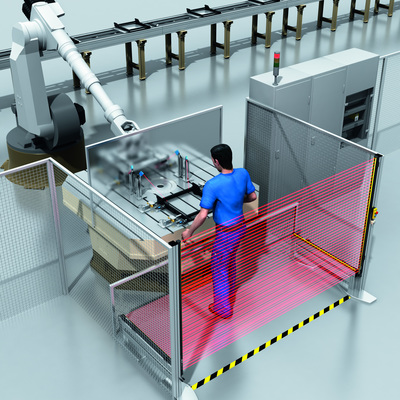
\includegraphics[scale=1.4]{coexistence}
	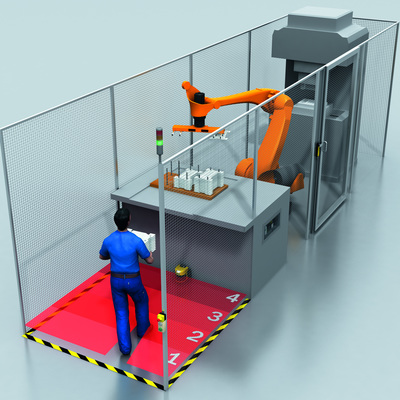
\includegraphics[scale=1.4]{cooperation}
	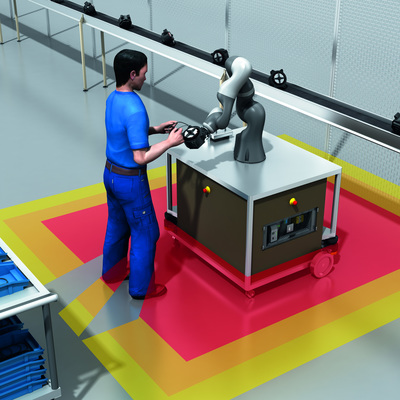
\includegraphics[scale=1.4]{collaboration}
	\caption[Caption for LOF]{Balról jobbra: együttes jelenlét, kooperáció, kollaboráció\footnotemark}
	\label{fig:coex-coop-collab}
\end{figure}

\footnotetext{Képek forrása: https://www.safetysolutions.net.au/content/machine/article/safety-solutions-for-intelligent-human-robot-collaboration-990038334}

\subsubsection{Biztonsági szempontok ember-robot kollaboráció esetén}
A biztonságos ember-robot együttműködés érdekében az elmúlt években különböző stratégiák lettek kifejlesztve. Ezek a módszerek különböző biztonságtípusra építenek, többek közt:
\begin{itemize}
	\item az ütközésbiztonság érdekében csak `biztonságos'/kontrollált ütközésre kerülhet sor robotok, emberek és akadályok között. Az emberekre gyakorolt erő/nyomaték határolása a fő szempont.
	\item aktiv biztonsági rendszer az ember és a berendezés közötti közelgő ütközések időben történő észlelése és a műveletek megállítása ekkenőrzött módon.
\end{itemize}











Ember és robot együttműködése (HRC - \angol{Human-Robot Collaboration}) egy olyan munkakörülmény, amely esetében az ember és a robot osztozik egyazon munkaterületen, egyazon időben. 

\end{document}
%---------------------------------------------------------

%--Tartalmi rész------------------------------------------
	%--Alkalmazáshoz szükséges műszaki feltételek elemzése
	\newpage
	\section{Alkalmazáshoz szükséges műszaki feltételek elemzése}

	%--Robotkar kalibráció, referenciafelvétel kidolgozása
	\newpage
	\documentclass[../documentation.tex]{subfiles}
 
\begin{document}
\section{Robotkar kalibráció, referencia felvétel kidolgozása}
Ha a robotkarhoz szerszámokat szeretnénk csatolni vagy a mozgását a térben elhelyzkedő tárgyakhoz szeretnénk igazítani, akkor kalibrációs eljárásokat kell végrehajtani.

\subsection{Koordinátarendszerek}
Ha a robotkar pozíciójáról beszélünk, akkor elsősorban a végpontjának vagy az arra szerelt szerszámnak a pozíciójára és orientációjára vagyunk kiváncsiak. Az ilyen elhelyezkedést a térben különböző koordinátarendszerekkel és a közöttük felírható transzformációkkal tudjuk jellemezni. A főbb koordinátarendszereket foglalja össze \aref{tab:coordsystems} táblázat.

\begin{figure}[h]
	\centering
	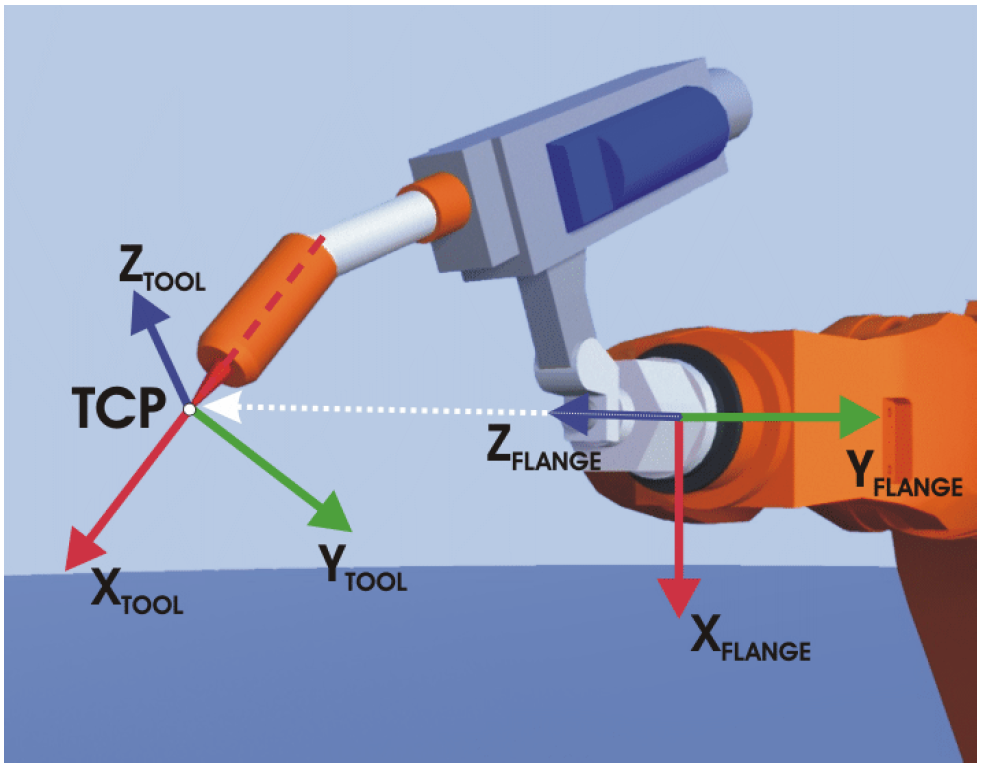
\includegraphics[scale=0.40]{tcp-calibration}
	\caption{A TCP (\angol{Tool Center Point}) elhelyezkedése\cite{sunrisemanual}}
	\label{fig:tcp-calibration}
\end{figure}

Ahhoz hogy egy test pozícióját és orientációját definiálni tudjuk a térben legalább 6 lineárisan független koordinátára van szükség. A viszonyítási koordinátarendszerben felírt 3 transzlációs és 3 rotációs koordináta megfelel erre a célra.
\begin{itemize}
	\item Transzlációs vektorok:
	\begin{itemize}
		\item X távolság: a referencia KR X tengelye mentén vett transzláció
		\item Y távolság: a referencia KR Y tengelye mentén vett transzláció
		\item Z távolság: a referencia KR Z tengelye mentén vett transzláció
	\end{itemize}
	\item Rotációs vektorok:
	\begin{itemize}
		\item A szög: a referencia KR Z tengelye körül vett forgatás
		\item B szög: a referencia KR Y tengelye körül vett forgatás
		\item C szög: a referencia KR X tengelye körül vett forgatás
	\end{itemize}
\end{itemize}

\begin{table}[h]
\setlength\arrayrulewidth{1pt}
\begin{tabu} to\linewidth{| X[1.4,c,m] | X[3,l,m] |}
\hline
\rowfont{\bfseries\large} Koordinátarendszer (KR) & Leírás \\ \hline
Világ KR & A világ KR egy állandó, Descartes-i (Cartesian) koordinátarendszer. Ez minden más KR gyökere, mint például a bázis KR-é vagy a robot bázis KR-é. Alapértelmezetten a világ KR a robot bázispontjában található. \\ \hline
Robot bázis KR & A robot bázis KR-e olyan Descartes-i KR, amely a robotkar bázispontjában található. Ez definiálja a robotkar relatív helyzetét a világ KR-hez képest. Alapértelmezetten a robot bázis KR megegyezik a világ KR-rel. Meg lehet adni egy elforgatási vektort a Sunrise.Workbench-ben, amely definiálja a robot relatív forgatását a világ KR-hez képest. Alapbeállítésként a padlóra rögzített robot felszerelési orientációja: (A=0°, B=0°, C=0°).\\ \hline
Bázis KR & Ahhoz hogy a Descartes-i térben mozgásokat definiálhassunk szükség van referencia KR (bázis) felvételére. Sztenderd módon a világ KR a mozgás bázis KR-e. További bázis KR-eket lehet definiálni a világ KR-hez képest. Ezt mutatja be \aref{sec:basecalibration}. fejezet. \\ \hline
\angol{Flange} KR & A flange KR írja le a robot \angol{flange} középpontjának a pozícióját és orientációját. Ennek az elhelyezkedése nem fix, a robottal együtt mozog. A \angol{flange} KR használható a rá fogatott szerszámokhoz kötődő KR-ek origójaként. Például a szakdolgozat keretében a gripper egy jól definiált pontjára illesztett KR a robot \angol{flange} KR-éhez kepést relatív lett megadva (\ref{fig:tcp-calibration} ábra). \\ \hline
Szerszám KR & A szerszám KR az a Descartes-i KR, amely a felszerelt szerszám munkapontjára illeszkedik. Ezt hívják szerszám középpontnak (\angol{Tool Center Point} - \textbf{TCP}). Bármennyi frame-et lehet definiálni egy szerszámhoz és ezek mindegyike kiválasztható TCP-nek. A szerszám KR rendszerint a \angol{flange} KR-ből származtatott. \\ \hline
\end{tabu}
\caption{A főbb koordinátarendszerek}
\label{tab:coordsystems}
\end{table}

\begin{figure}
	\centering
	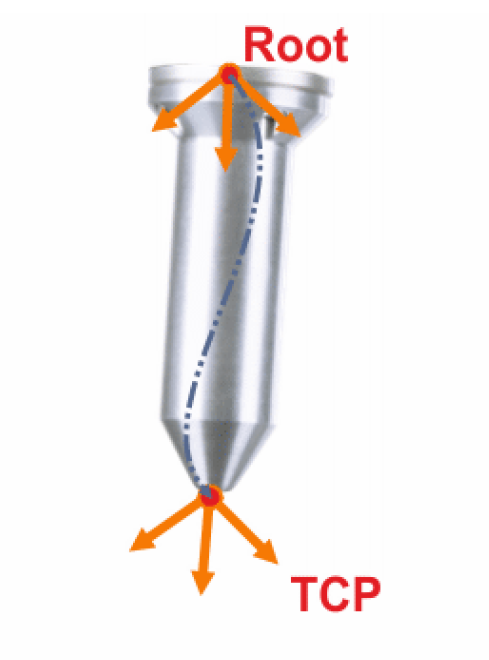
\includegraphics[scale=0.35]{tcp-example1}
	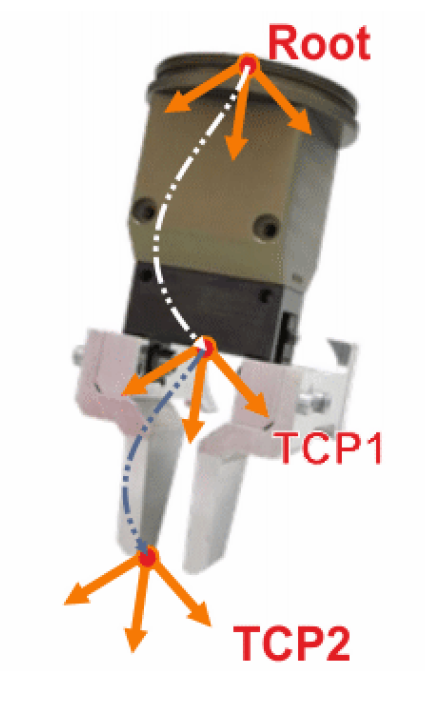
\includegraphics[scale=0.35]{tcp-example2}
	\caption{Szerszám 1 (balra) és 2 (jobbra) TCP-vel\cite{sunrisemanual}}
	\label{fig:tcp-examples}
\end{figure}

\newpage
\subsection{Szerszámkalibráció - XYZ 4-pont metódus}
A sakkprojekt kivitelezése során szükséges a robotkarra szerelt megfogó kalibrálása ahhoz, hogy a pozícionálás minél pontosabb legyen. A robotkar szoftverében ez egy alapfunkció, kiegészítő csomag nem szükséges hozzá. A kalibrációs eljárás alapvetően 2 lépésből áll:
\begin{enumerate}
	\item a TCP origójának meghatározásból,
	\item az origóra illesztett koordinátarendszer orientálásából.
\end{enumerate}
A második lépés jelen esetben elhagyható, megfelelő ha a TCP az orientációját a referencia KR-től örökli. 

A TCP origójának meghatározására használt módszer: XYZ 4-pont metódus. Ehhez ki kell választanunk a szerszám egy adott pontját adott helyzetben (pl.: gripper egyik csúcspontja nyitott állásban); ez lesz a TCP. Az eljárás lényege, hogy a kalibrálni kívánt szerszám ezen pontját egy referenciaponthoz vezéreljük 4 különböző irányból. A referencia pont szabadon választható. A robot kontroller a különböző \angol{flange} pozíciókból számolja ki a TCP helyzetét.

A 4 \angol{flange} pozíció egymás közötti távolságainak meg kell haladniuk egy előre definiált minimumot. Ha a pontok túl közel vannak egymáshoz, akkor a pozíció adatokat nem lehet elmenteni. Erre hibaüzenet figyelmeztet.

A kalibráció minősége a transzlációs vektor hibájával mérhető, amit a program kalibráció közben számít ki. Ha ez a hiba meghalad egy definiált határértéket, akkor célszerű a TCP-t újból kalibrálni.

A minimális távolságok és a maximális számítási hiba a \angol{Sunrise Workbench}-ben konfigurálható. Részletesebb leírás az eljárásról a megfelelő Sunrise.OS verzió manuáljában található\cite{sunrisemanual}.

\begin{figure}[h]
	\centering
	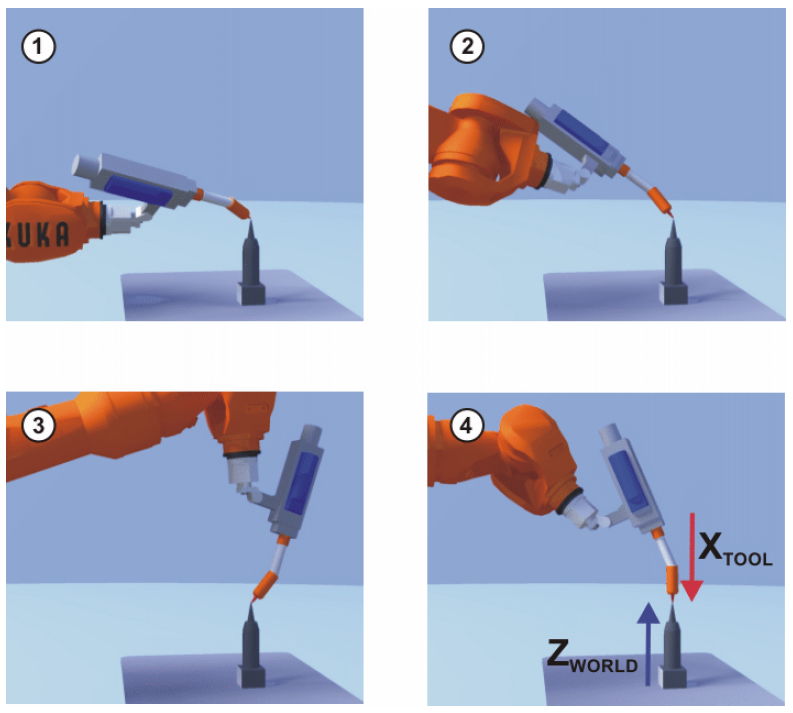
\includegraphics[scale=0.50]{tcp-calibration2}
	\caption{XYZ 4-pont metódus 4 lépése\cite{sunrisemanual}}
	\label{fig:tcp-examples}
\end{figure}

\subsection{Báziskalibráció - 3 pont metódus} \label{sec:basecalibration}
A báziskalibráció során a felhasználó egy Descartes-i koordinátarendszert (bázis koordinátarendszert) rendel a bázisnak választott frame-hez. A bázis KR-nek a felhasználó által választott, tetszőleges helyen lehet az origója.

A bázis kalibráció előnyei:
\begin{enumerate}
	\item A TCP végigvezérelhető a munkafelület szélein vagy egy munkadarabon.
	\item A bázishoz viszonyítva lehet felvenni a szükséges pontokat. Ez a szakdolgozat során azért fontos, mert így nem kell a sakktábla egyes mezőihez tartozó pontokat külön felvenni, a pozíciókat meg lehet adni a bázisponthoz képest, ami lehet például a sakktábla egyik sarokpontja.
\end{enumerate}

A 3-pont metódus során az origó és a bázis 2 további pontja kerül rögzítésre. Az origó felvétele után a kívánt X tengely pozitív felén egy tetszőleges pont rögzítése következik. Végezetül az XY sík első térnegyedébe eső, szintén tetszőlegesen választott pontot kell felvenni. Ez a 3 pont egyértelműen meghatározza a bázist.

A rögzített pontok origótól vett távolságának meg kell haladnia egy minimumot, illetve az egyenesek között is meg kell lennie egy minimum szögnek (origó - X tengely és origó - XY síkon felvett pont). Ha a pontok túl közel vannak vagy az említett szőgek túl kicsik, akkor a pozíció adatokat nem lehet elmenteni. Erre hibaüzenet figyelmeztet.

A minimális távolságok és szögek a \angol{Sunrise Workbench}-ben módosíthatók. Részletesebb leírás az eljárásról a megfelelő Sunrise.OS verzió manuáljában található\cite{sunrisemanual}.

\begin{figure}[h]
	\centering
	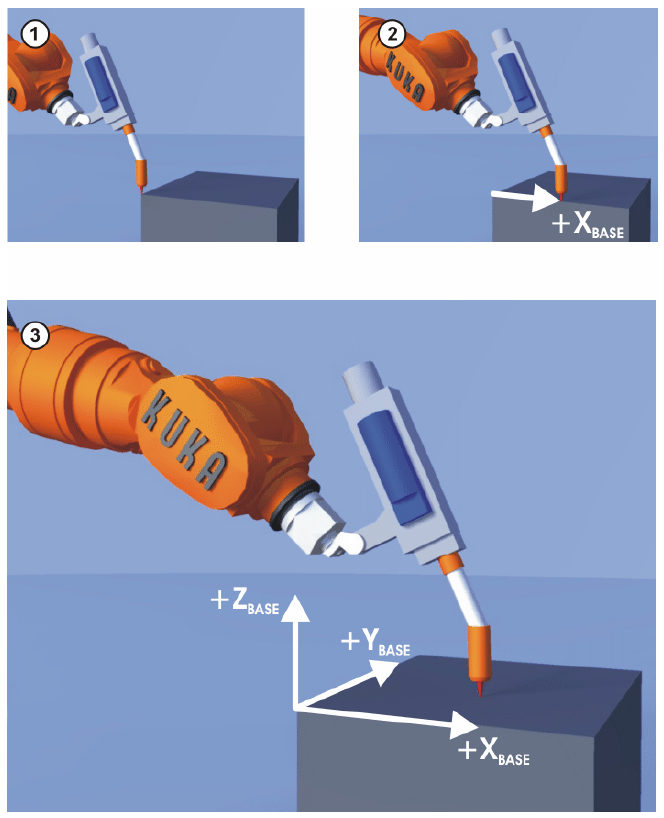
\includegraphics[scale=0.50]{basecalibration}
	\caption{Báziskalibráció 3-pont metódussal\cite{sunrisemanual}}
	\label{fig:basecalibration}
\end{figure}

\subsection{A szerszám tömegeloszlásának meghatározása}
A robotkaron tengelyeiben ébredő többlet nyomatékra meg lehet határozni egy maximális értéket, így ha a munkaterében lévő objektummal ütközik, detektálja és megáll. A robot saját tömegének dinamikus mozgatásához szükséges nyomatéka nem adódik hozzá ehhez a többlet nyomatékhoz. Adott szerszám robotkarra erősítésével viszont előfordulhat, hogy a maximális járulékos nyomatékérték átlépi valamelyik tengelyen a megengedett nyomatékértéket. Ezen hatás korrigálásához szükséges a szerszám tömegeloszlásának kalibrálása (a sakkbábuk, mint munkadarabok kalibrálása nem szükséges, azok tömege elhanyagolható).

A tömegeloszlás meghatározásához a robot először különböző méréseket futtat automatikusan a csuklótengelyek (utolsó három tengely: A5, A6, A7) mozgatásával. Ez alapján a robotkarra szerelt szerszám tömege és a tömegközéppontjának helye meghatározható. Másik lehetőség a szerszám tömegének megadása (például katalógus alapján), majd ez alapján a tömegközéppont helyének kalibrálása.

Az eljárás futtatásához nincs szükség plusz csomagra, a funkció a robotszoftver beépített eleme. A lépések a következők (automatikusan történik, a folyamat 1-2 percet vesz igénybe):
\begin{enumerate}
	\item A folyamat kezdetén az A7 tengelyt a vezérlő a 0 pozícióba mozgatja. Ezen kívül az A5 tengelyt úgy pozícionálja, hogy az A6-os tengelyre többletnyomatékot a súly ne fejtsen ki. Ekkor a szerszám tömegközéppontja abba a síkba esik, amit az A6 tengely és a gravitációs térerősségvektor kifeszít.
	\item A mérés futása során az A6 és az A7 tengelyek egy bizonyos tartományban vesznek fel helyzeteket:
	\begin{itemize}
		\item Alapbeállításként az A6 tengely -95° és +95° közötti vesz fel pozíciókat.
		Ha a munkatér nem elég nagy ehhez a mozgástartományhoz, akkor ez a tartomány csökkenthető.
		\item Az A7 tengely 0°és -90° között mozog.
	\end{itemize}
\end{enumerate}

A mérést befolyásoló tényezőkről információ a Sunrise kézikönyvében\cite{sunrisemanual} található.

\begin{figure}[h]
	\centering
	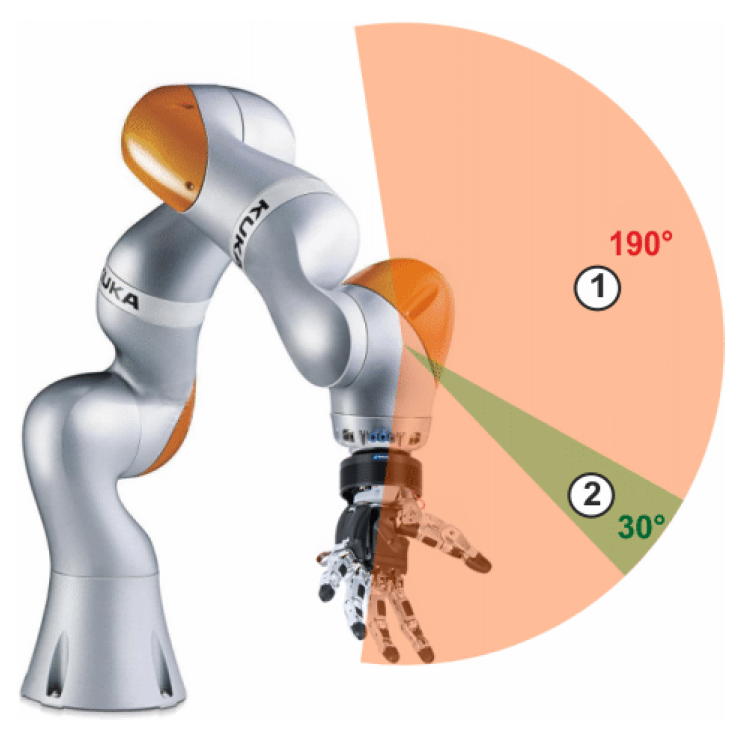
\includegraphics[scale=0.50]{loaddatacalibration}
	\caption{Az A6 tengely mozgástartománya: 1-es esetben teljes, 2-es esetben csökkentett tartomány\cite{sunrisemanual}}
	\label{fig:loaddatacalibration}
\end{figure}

















\end{document}
	%--Robotkar mozgásának definiálása és programozása
	\newpage
	\documentclass[../documentation.tex]{subfiles}
 
\begin{document}
\section{Robotkar mozgásának definiálása és programozása}
\subsection{Biztonsági beállítások}
Ahhoz hogy a robot működése során ne jelentsen veszélyt a munkaterében lévő emberekre és vagyontárgyakra, különböző biztonsági eszközök beszerelésére, illetve akitválására van szükség. A robotszoftverben implementált biztonsági funkciók között vannak módosítható és permanens elemek. Ezeket foglalja össze felsorolás jelleggel \aref{sec:safetyfunctions} fejezet. A továbbiakban csak a projekt során is aktív elemek kerülnek tárgyalásra.

\subsubsection{Vészleállító eszköz}
Az ipari robot esetében a vészleállító eszköz (\angol{EMERGENCY STOP	 device}) a smartPAD-en található vészleállító (\ref{fig:smartpad} ábra). Ezt a kapcsolót kockázatos szituációban vagy vészhelyzetben kötelező benyomni.

Ha az operátor benyomta a vészleállító gombot, akkor a robotkar \angol{Safety stop 1 (path-maintaining)} (leírás \aref{tab:terms} táblázatban) megállást hajt végre. Az EMERGENCY STOP eszközt el kell csavarni ahhoz, hogy a műveletek folytatódhassanak.

\subsubsection{Engedélyező eszköz}
A robotkar esetében az engedélyező eszközök (\angol{enabling devices}) a smartPAD-re szerelt engedélyező kapcsolók. 3 ilyen kapcsoló található a smartPAD-en (\ref{fig:smartpad} ábra). Ezek mindegyikének 3 állása van:
\begin{itemize}
	\item Nem behúzott
	\item Középső pozíció
	\item Teljesen behúzott (pánik pozíció)
\end{itemize}

A teszt módokban és CRR esetén (\ref{tab:terms}) a robotkar csak akkor mozgatható, ha legalább 1 engedélyező kapcsoló középső állásban van.
\begin{itemize}
	\item Az engedélyező kapcsoló elengedése \angol{Safety stop 1 (path-maintaining)} megállást fog okozni.
	\item A kapcsoló teljes behúzása is ugyanilyen megálláshoz vezet.
	\item 2 engedélyező kapcsolót a középső pozícióban tartani lehetséges néhány másodpercig. Ez lehetőséget ad arra, hogy az operátor fogást váltson. Ha 2 engedélyező kapcsoló párhuzamosan középső pozícióban van tartva 15 másodpercnél tovább, az szintén \angol{Safety stop 1 (path-maintaining)} megállást fog okozni.
\end{itemize}

Ha az engedélyező kapcsoló a középső állásban ragad, akkor a következő lehetőségek állnak rendelkezésre:
\begin{itemize}
	\item a kapcsoló teljes behúzása,
	\item az EMERGENCY STOP eszköz benyomása,
	\item illetve a Start gomb elengedése
\end{itemize}

\begin{figure}[h]
    \centering
    \begin{subfigure}[t]{0.5\textwidth}
        \centering
        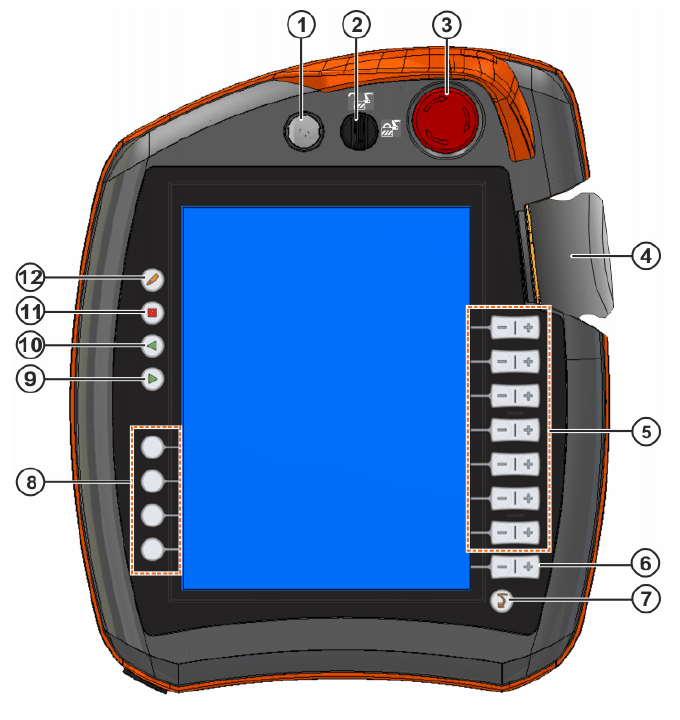
\includegraphics[scale=0.4]{smartpad-front}
        \caption{smartPAD előlnézetből\\ 2: kulcsos kapcsoló\\ 3: EMERGENCY STOP eszköz \\ 9: Start gomb}
    \end{subfigure}%
    ~ 
    \begin{subfigure}[t]{0.5\textwidth}
        \centering
        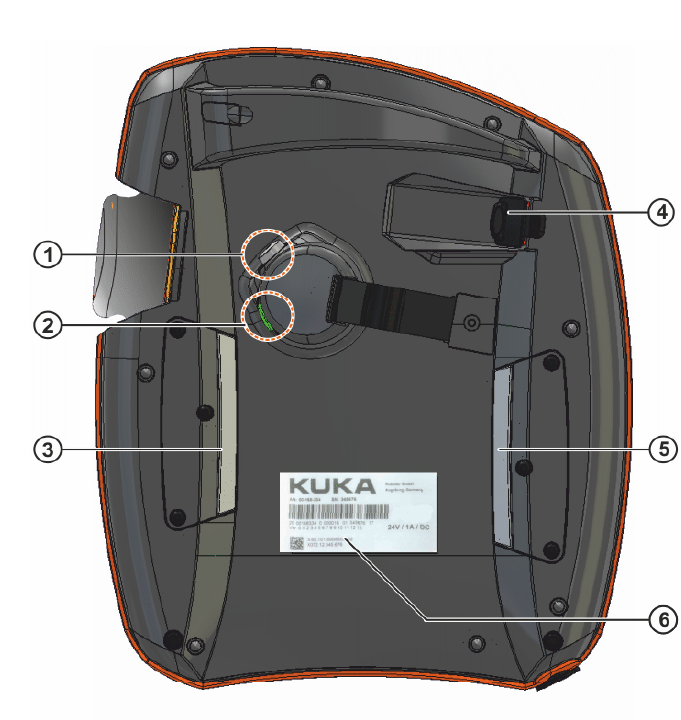
\includegraphics[scale=0.4]{smartpad-rear}
        \caption{smartPAD hátulnézetből\\ 1, 3, 5: enegedélyező kapcsoló\\ 2: Start gomb}
    \end{subfigure}
    \caption{KUKA smartPad\cite{sunrisemanual}}
    \label{fig:smartpad}
\end{figure}

\subsubsection{Operációs mód rögzítése}
Ahhoz hogy a robot mozgása közben ne lehessen operációs módot váltani (pl.: T1 módból T2-be), a smartPAD-en található egy kulcsos kapcsoló (\ref{fig:smartpad} ábra). Ennek elfordítására a robot megáll, ekkor lehet tetszőleges operációs módot választani. Ezeket \aref{tab:terms} táblázat részletesen tartalmazza.

\subsubsection{Megállást előidéző események}
A sakkprojekt során az alábbi események megállást idézhetnek elő a program futása során (a csillagozott elemek permanensen a robotszoftverbe vannak programozva, ezeket módosítani nem lehet):
\begin{itemize}
	\item operációs mód váltás történt mozgás közben*,
	\item az engedélyező kapcsolót elengedték*,
	\item az engedélyező kapcsolót teljesen behúzták*,
	\item a smartPAD-en található \angol{EMERGENCY STOP} eszközt benyomták*,
	\item a tengelyekre előírt maximális többletnyomatékot valamelyik tengelyen meghaladja a terhelés.
\end{itemize}

\subsection{Mozgástípusok elméletben}
Ez a fejezet bemutatja a mozgások programozásának elméleti szabályait. A szakdolgozat során programozott elemeket \aref{sec:motionprogramming} fejezet tárgyalja.

\subsubsection{Mozgástípusok áttekintése}
Több egymás utáni mozgás végrehajtása során a mozgás kezdőpontja mindig az előző végpontja.
A következő mozgástípusokat lehet beprogramozni különálló mozdulatokként:
\begin{itemize}
	\item Point-to-point (PTP, Ponttól pontig)
	\item Lineáris mozgás (LIN)
	\item Körkörös mozgás (\angol{Circural motion}, CIRC)
	\item Manuális vezetés kézi vezető eszközzel
\end{itemize}

A következő mozgástípusokat lehet beprogramozni a CP (``\angol{Continuous Path}'' - ``folytonos út'') spline\footnote{A mozgatott pont spline mentén halad a térben} blokk\cite{sunrisemanual} részeként:
\begin{itemize}
	\item Lineáris mozgás (LIN)
	\item Körkörös mozgás (\angol{Circural motion}, CIRC)
	\item Polinomiális mozgás (SPL)
\end{itemize}

JP (``\angol{Joint Path}'' - ``tengely út'') spline\footnote{Mivel a robotkar 7 tengellyel rendelkezik, a mozgása közben a tengelyek állása nem egyértelmű. JP sline blokk kivitelezésénél a tengelyek szögsebessége folytonos, így egy kedvezőbb dinamikájú mozdulatsort visz véghez.} blokk\cite{sunrisemanual} programozásakor PTP elemeket lehet használni.

A LIN, CIRC, SPL, CP spline blokk mozdulatok CP (``\angol{Continuous Path}'') típusúak, míg a PTP és a JP spline blokk JP (``\angol{Joint Path}'' - ``tengely út'') típusúak.

\subsubsection{PTP mozgástípus}
A robot a TCP-t a leggyorsann úton vezeti el a végponthoz. A leggyorsabb út általában nem egyezik meg a térbeli legrövidebbel, tehát nem egy egyenes (\ref{fig:ptpmotion}). A görbe útvonalak lekövetése gyorsabb az egyenesnél, mivel a robot tengelyei forogva és szimultán mozognak.

PTP a gyors pozícionáló mozgás. A mozgás pontos útvonala nem előre megjósolható, de többszöri futtatásra is ugyanazt az útvonalat követi le, feltéve ha az általános feltételek nem változtak.

\begin{figure}[h]
    \centering
    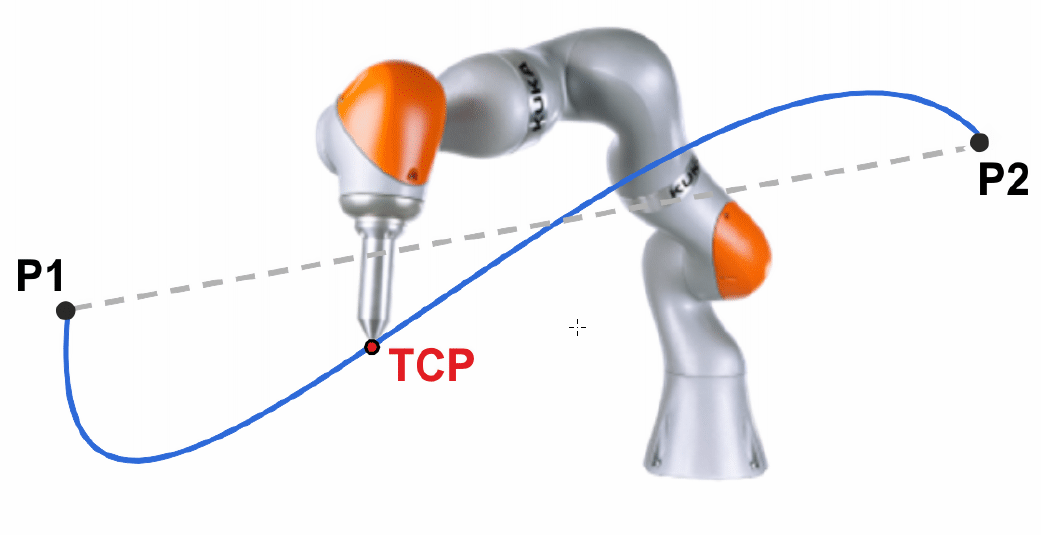
\includegraphics[scale=0.4]{ptpmotion}
    \caption{PTP mozgás\cite{sunrisemanual}}
    \label{fig:ptpmotion}
\end{figure}

\subsubsection{LIN mozgástípus}
A robot a TCP-t egy térbeli egyenes mentén mozgatja a végponthoz. A LIN mozgás során a végpozíció konfigurációját a program nem veszi figyelembe.

\begin{figure}[h]
    \centering
    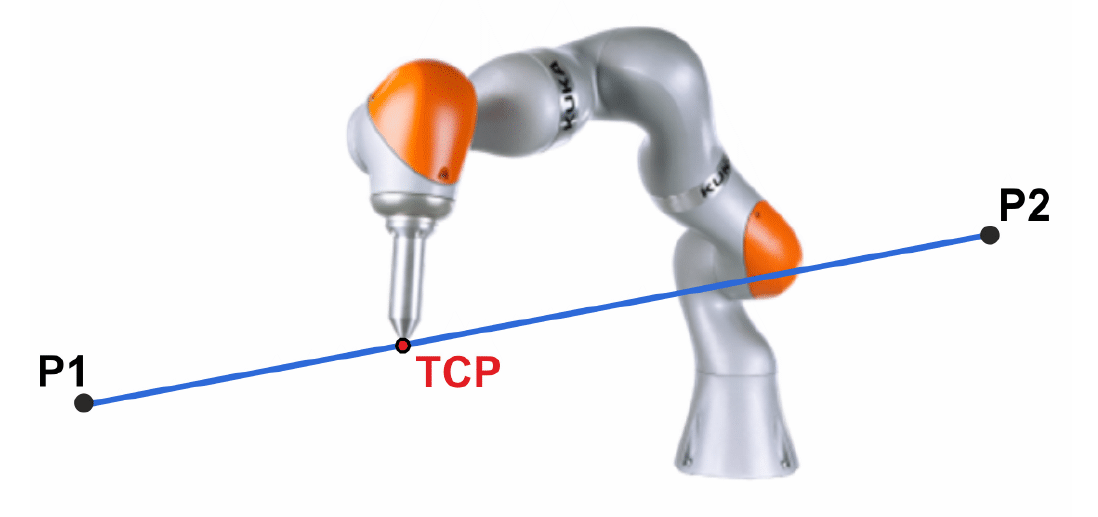
\includegraphics[scale=0.4]{linmotion}
    \caption{LIN mozgás\cite{sunrisemanual}}
    \label{fig:linmotion}
\end{figure}

\newpage
\subsection{A robotkar mozgatása} \label{sec:motionprogramming}
A projekt során a robotkarral egyszerű mozgásokat kellett végeztetni. Nem volt szükség bonyolultabb görbék és felületek lekövetésére, csak ponttól ponttig mozgásra.

A robot mozgása szekvenciálisan ismétlődik, ennek lépései a következők:
\begin{enumerate}
\setcounter{enumi}{-1} 
	\item a robotkar képfelvételi pozícióba vezérlése (a normál játékmenet közben mindig ebből a pozícióból indul, nem kell ide irányítani)
	\item a sakkprogram által meghatározott lépés kezdőmezője fölé irányítása
	\item csökkentett sebességgel a bábuért lenyúlás, majd a gripper záródása után szintén csökkentett sebességgel visszaemelés
	\item a lépés végpontja fölé vezérlés
	\item redukált sebességgel a bábu lerakása, majd a gripper kinyílása után szintén redukált sebességgel visszaemelkedés a bábu fölé
	\item képkészítési pozícióba való visszatérés
\end{enumerate}

A szakdolgozat keretében megírt program nem keresi meg automatikusan az ideális képkészítési pozíciót (továbbfejlesztési irány), ezt kézzel kell megtennünk. Erre a csuklók direkt vezérlése is alkalmas, de praktikusabb egy tetszőleges koordinátarendszerben XYZ tengelyek mentén mozgatni (például a sakktábla sarkán felvett bázis KR-ben).

Ahhoz hogy a kamera látóterébe az egész kalibrációs tábla beleessen a robotkarnak viszonylag magasra kell nyúlnia. Ezt a 7, illetve a 14 kilós iiwa robotkar mozgástere is megengedi. Kisebb méretű robottal a projekt megvalósításához nagyobb látószögű kamerára vagy több képkészítési pozícióra lenne szükség.

\begin{figure}[h]
    \centering
    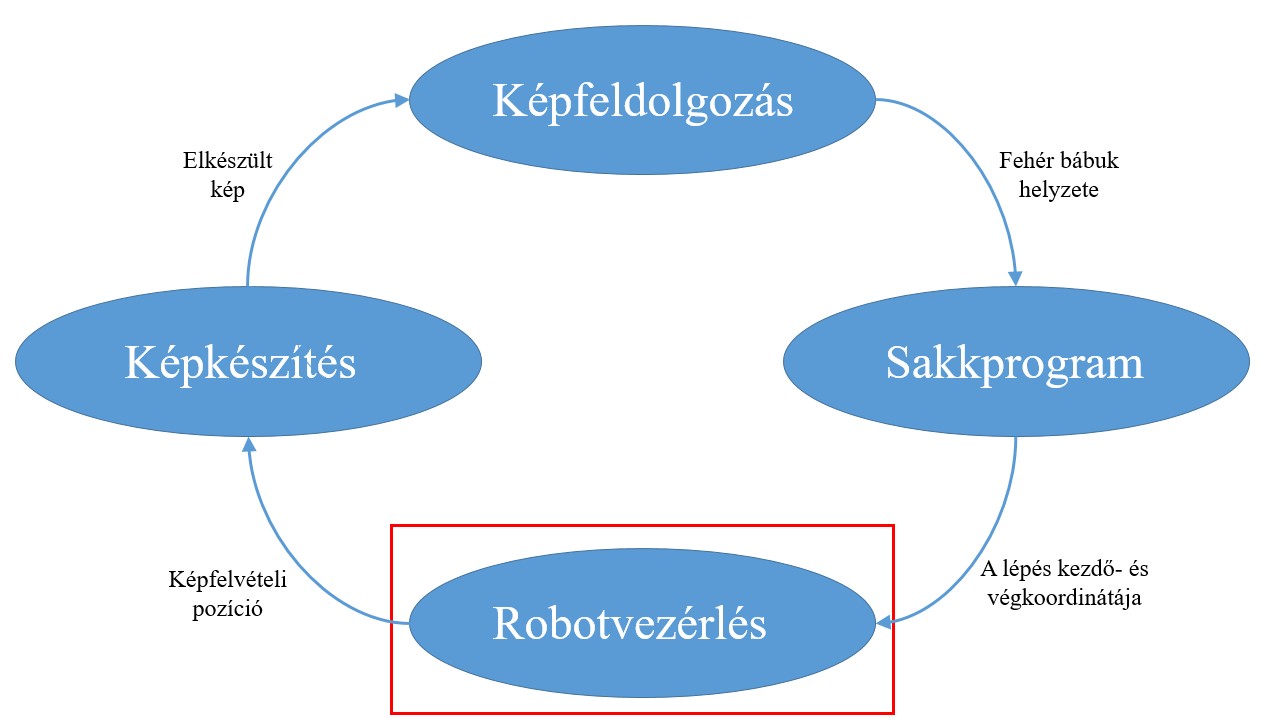
\includegraphics[scale=0.4]{flowchart-robot}
    \caption{A robotvezérlés helye a folyamatban}
    \label{fig:flowchart-robot}
\end{figure}

Praktikus lehet egy olyan frame betanítása, ahol az orientáció olyan, ahogy a robotkarnak a bábut meg kéne fognia. Erről a frame-ről másolatot készítve annak X, Y és Z koordinátáját külön-külön be lehet állítani. A sakktábla bázispont és ez a frame alapján a tábla összes mezőjéhez lehet generálni egy alsó megfogó helyzetet (ahol a megfogó két pofája összezáródik) és egy felsőt, ahová a képkészítés után megy. Az alsó megfogó helyzet a gripper TCP-re vonatkozik, a robotkar mozgatásához célszerű ezt a pontot irányítani.

A hagyományos sakktábla 8x8-as, az alsó és felső pozíciót is beleszámolva ez 128 generált frame-et jelent. Ezek kiszámítása nem különösebben időigényes, de áttekinthetőbb a programkód, ha ezekből a fizikai pozíciókból a sakkprogramhoz hasonlóan egy (az alsó és felső helyzet miatt 2) 8x8-as tömböt építünk fel a sakkprogramhoz hasonló indexeléssel. Mivel a sakktábla méretei ismertek, ezt 2 egymásba ágyazott for ciklussal meg lehet oldani, a bázis koordinátarendszerhez a megfelelő offszetet hozzáadva.

A projekt során a megfogópofa egyik sarokpontja lett betanítva TCP-nek, így szükség van még egy plusz offszetre ahhoz, hogy a robotkar mozgatásakor a megfogó középvonala kerüljön a mező közepe fölé, ne pedig a TCP (\ref{fig:tcp-examples} ábra).

A bábuk mozgatására érdemes külön függvényt írni, ami fogadja a sakkprogram által visszaadott kezdő- és végpont indexeket, majd ez alapján az adott bábut áthelyezi a megfelelő mezőre. A főprogramban implementált `MovePiece' függvény ezt a célt szolgálja. A bábuk emelésekor és letételekor érdemes a PTP mozgatás helyett a LIN-t alkalmazni, mivel annak tetszőlegesen állítható a sebessége\footnote{A PTP esetén is meg lehet adni egy százalékos sebességredukciót a tengelyekre.}.










\end{document}
	%--Sakkalgoritmus beágyazása
	\newpage
	\documentclass[../documentation.tex]{subfiles}
 
\begin{document}
\section{Sakkalgoritmus beágyazása}
A robotprogramhoz felhasznált sakkalgoritmusok és főbb Java osztályok alapja egy versenyre készített, nyílt forráskódú sakk alkalmazás \cite{chessgui}. 2005-ben Arwid (Arvydas) Bancewicz első helyezést ért el ezzel az alkalmazásával az OBEA Számítógépes Programozó Versenyen (\angol{OBEA Computer Programming Contest}) 17 évesen. Az általa készített program rendelkezik grafikus felhasználói felülettel (továbbiakban GUI - \angol{Graphical User Interface}), a forráskód nagy része ennek megfelelő működtetéséhez lett megírva.

A szakdolgozat keretében megvalósított projektem során külön a sakk alkalmazáshoz felhasználói felületet létrehozni nem volt szükségszerű. A robotprogram továbbfejleszthető olyan formában, hogy folyamatosan kijelezze a jelenlegi sakkállást, így még inkább nyomon követhető a játék menete, így megkönnyítve a továbbfejlesztést. Ezen a felületen keresztül akár tetszőleges felállást lehetne konfigurálni a játék kezdetéhez.

A sakkprogram beágyazásának első fő kihívása a GUI elhagyásával egy konzolalkalmazás létrehozása. A program forráskódja viszonylag hosszú, sok osztály lett implementálva különböző csomagokba rendezve (12 csomag és ezeken belül 93 osztály). A program működésének megértéséhez jó kiindulási pont a mellékelt README fájl és a ``\angol{program documentation}'' mappában található szotver leírás (\angol{Software Documentation.doc})\cite{chessgui}. Habár ezek főként a GUI működését taglalják, az ehhez tartozó főprogram kódjából a meghívott függvények alapján ki lehet következtetni a működés struktúráját. Ezen felül a Java osztályoknak és az egyes csomagoknak beszédes nevük van, például a következő sakklépést az \angol{algorithm} (algoritmus) csomagban található különböző algoritmusokra alapozott osztályok metódusai határozzák meg.

A szakdolgozathoz felhasznált csomagok az alábbiak (ezeken belül is bizonyos funkciók ki lettek kapcsolva, de ezek jelentik a program magját):
\begin{itemize}
	\item chess.algorithm: Ebben a csomagban kerültek implementálásra a különböző sakkalgoritmusokat meghívó és végrehajtó utasítások. Ezen felül itt lettek implementálva az bábuk lehetséges lépései.
	\item chess.core: Ez a csomag tartalmazza a sakkhoz szorosan kötődő osztályokat, metódusokat (pl.: bábuk elhelyezkedése a táblán).
	\item chess.properties: Itt találhatóak a programozott sakkjáték szempontjából praktikus funkciók (pl.: játék jelenlegi állása, játékosok neve stb.).
\end{itemize}

\subsection{A chess.algorithm csomag - az algoritmusok működtetője}
A programban az alábbi sakkalgoritmusok lettek implementálva:
\begin{itemize}
	\item Alfa-béta vágás (AlphaBeta.java)
	\item Minimax elv (MiniMax.java)
	\item NegaScout algoritmus (NegaScout.java)
	\item Principal variation search (PrincipalVariation.java)
	\item Kvázi véletlenszerűen választott szabályos lépés (RandomGen.java)
\end{itemize}

A sakkprogram alapbeállításként az Alfa-béta vágást használja. Az Alfa-béta vágás egy olyan kereső algoritmus, amely igyekszik csökkenteni a minimax algoritmus keresési fájában lévő kiértékelt elemek számát. Ezt a módszert gyakran alkalmazzák kétszemélyes játékok (pl.: amőba, sakk, go, stb.) esetén gépi játékos programozására. Egy adott lépés kiértékelését akkor szakítja meg teljesen, ha legalább egy válaszlépés bebizonyítja, hogy a lépés rosszabb, mint a korábban vizsgált lépés. Az ilyen lépések további vizsgálata felesleges. Ha egy hagyományos minimax fára alkalmazzák, akkor ugyanazt a lépést adja majd vissza, mint amit a minimax algoritmus adna, de kimetszi azokat az ágakat a fában, amik a kimenetet nem befolyásolják.\footnote{Szöveg forrása angol nyelven: https://en.wikipedia.org/wiki/Alpha\%E2\%80\%93beta\_pruning}

\begin{figure}[h]
\centering
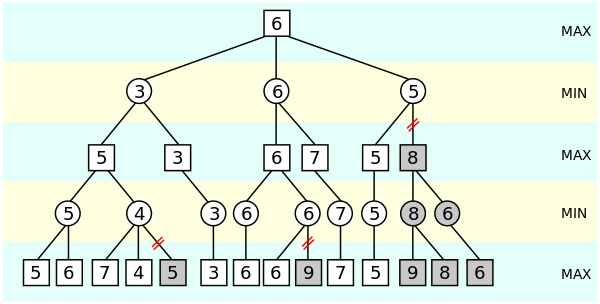
\includegraphics[scale=0.55]{alphabeta}
\caption{Az alfa-béta vágás szemléltetése. A kiszürkített részfák vizsgálata felesleges (a lépések jobbról balra történő kiértékelésekor). A max és min szintek reprezentálják a játékos, illetve az ellenfelének a lépéseit. \protect\footnotemark}
\label{fig:alphabeta}
\end{figure}
\footnotetext{A kép forrása: https://upload.wikimedia.org/wikipedia/commons/thumb/9/91/\\AB\_pruning.svg/600px-AB\_pruning.svg.png}

Az algoritmus két változót értékel ki minden lépésben, alfát és bétát. Az alfa érték reprezentálja azt a minimum pontszámot, amely az u.n. `maximalizáló' játékos számára már biztosítva van, illetve a béta érték az a maximum pontszám, ami az u.n. `minimalizáló' játékos számára biztosított. Kezdetben alfa értéke negatív végtelen, béta pozitív végtelen, azaz mindkét játékos a saját legrosszabb lépésével indít. A fa rekurzív vizsgálata során folyamatosan változik az értékük a játékosok által garantáltan elérhető értékekre. Amint a béta érték az alfa alá csökken az azt jelenti, hogy ez az állás (ha mindkét játékos részéről a legjobb lépéseket tételezzük fel) nem állhat elő, így további vizsgálatuk felesleges.

Az algoritmusokat a sakk szabályaihoz és sajátosságaihoz a MoveAlgorithm illeszti. Ez az osztály az alábbi funkciókat tartalmazza (egyéb kiegészítő, teszteléshez megírt függvényeken felül):
\begin{itemize}
	\item Definiálja az egyes bábuk lehetséges lépéseit mezőkre lebontva, tehát az erre vonatkozó metódusok pontosan megadják, hogy az egyes bábuk melyik mezőkről melyikekre léphetnek. Példának okáért a gyalog esetén külön a fehér bábukra és külön a feketékre is meg van határozva (getPawnMoves(Coord c) függvény), hogy a kiindulási pontjukról az ellenfél irányába egyet vagy kettőt is léphetnek. Bármely más esetben 1-et léphetnek előre (az ütéseket külön függvények definiálják, ezek elkülönítése a robotprogramozás esetén is kifejezetten előnyös).
	\item Az egyes bábuk lehetséges ütéseit külön függvények határozzák meg. A gyalog kivételével a többi bábunál ez megegyezik az előző pontban leírt lépésekkel.
	\item A bábuk játékhelyzettől függő összes lehetséges lépését, ütését a `getRealMoves', a `getRealAttacks' és a `getRealAll' függvények adják vissza. Ezek kizárján azon lépéseket, melynél az adott játékos királya a lépés előtt és utána is sakkban áll. Ezt úgy vizsgálja meg a program, hogy adott játékállásban ``meglépi'' a kívánt lépést, majd ellenőrzi, hogy a király sakkban maradt-e.
	\item Itt találhatóak még az egyes játékállások ``költségét'' meghatározó függvények, amelyek által visszaadott értékek az algoritmusok működtetésének alapjait jelentik.
\end{itemize}

\subsection{A chess.core csomag - a játék magja}
A chess.core csomag definiálja az algoritmusok működtetéséhez nem szorosan kapcsolódó osztályokat. A fő fájl a ChessGame.java, ennek segítségével lehet egy játékot elkezdeni. A példányosításakor az alábbi inicializáló lépések futnak le:

\begin{enumerate}
	\item A játék állapota inicializáltra változik (a játékállapotokról a chess.properties csomag kapcsán lesz bővebben szó).
	\item Alapértelmezetten az Alfa-béta kereső algoritmus kerül beállításra. Ezt a játék során bármikor lehet módosítani a `setAlgorithm' függvény segítségével.
	\item A játékosok neve alapértelmezetten ``Black'' és ``White'', ezt is bármikor lehet módosítani a játék közben. Kiindulásként a fehér játékos az ember, a fekete a robotkar, de a program viszonylag könnyedén átalakítható ha ezt meg szeretnénk cserélni.
	\item A hagyományos sakkjátszmák során a játékosok egy sakkórát (\ref{fig:chessclock} ábra) használnak arra, hogy maximalizálják a játék idejét. Mindkét játékosnak előre meghatározott és beállított ideje van a gondolkozásra. Ha az adott játékos lépett, lenyom az órán egy kapcsolót, melynek hatására a másik játékos ideje telik addig, amíg ő is vissza nem kapcsolja az órát. A program két virtuális órát használ erre a célra, melyek indítása és megállítása automatikusan történik minden lépésnél.
\begin{figure}[h]
\centering
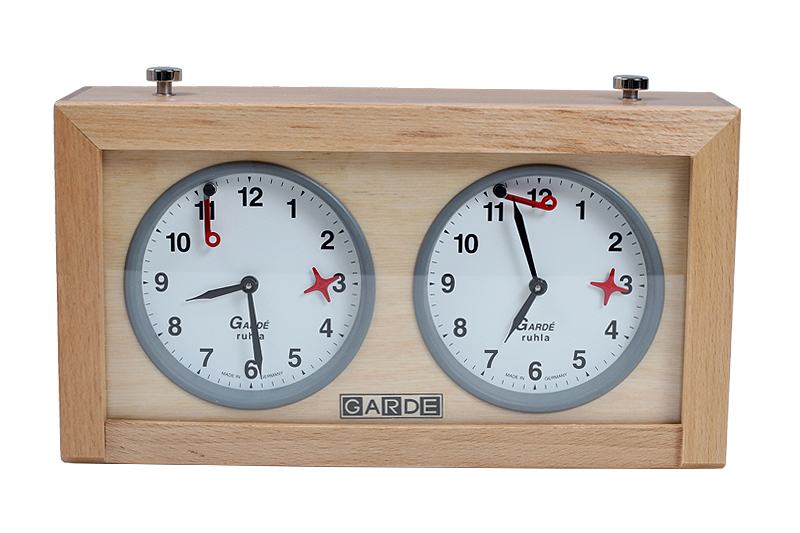
\includegraphics[scale=0.40]{chessclock}
\caption{Hagyományos játékokhoz használt sakkóra - a piros zászló leesése jelzi, ha a játékos ideje elfogyott \protect\footnotemark}
\label{fig:chessclock}
\end{figure}
\footnotetext{A kép forrása: https://www.polishchess.com/garde-analog-chess-clock-classic-p-161.html}
	\item A tábla és az alap felállás inicializálása a Board osztály példányosításával történik. Ez az osztály tartja számon, hogy melyik mezőn milyen bábu található, emellett praktikus okokból a két király jelenlegi helyzetét külön változókban tárolja.
\end{enumerate}

A bábuk pozíciója kapcsán külön érdemes kiemelni, hogy a pozíciót a bábuk koordinátája határozza meg. A lehetséges koordinátákat egy 8x8-as tömb jelképezi. A tömb [0,0] indexű eleme a tábla A1 mezője, a [7,7] pedig a H8 (\ref{fig:chessboard} ábra).

\begin{figure}[h]
\centering
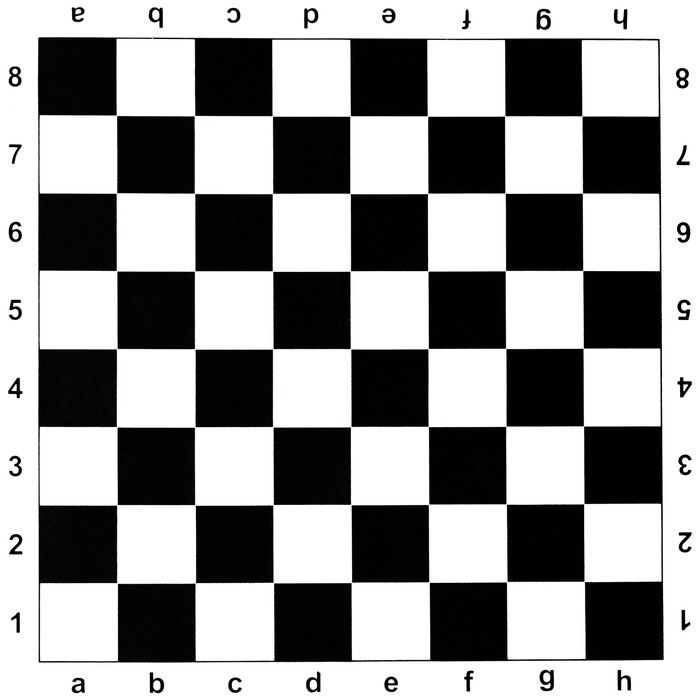
\includegraphics[scale=0.45]{chessboard}
\caption{A sakktábla mezőihez koordináták rendelése}
\label{fig:chessboard}
\end{figure}

Létrehozni lépést a Move osztály példányosításával lehet. A konstruktor egy kezdő és egy végponti $x$ és $y$ koordinátát vár, amelyek a bábu kiindulási- és végkoordinátái. Azt, hogy egy lépés szabályos volt-e úgy lehet ellenőrizni, hogy meghívjuk a sakkjáték példányunk `checkIfLegalMove' függvényét paraméterként átadva a lépést. Fontos, hogy a jelenlegi sakkjáték példányunkra hívjuk meg ezt a metódust, így biztos a pillanatnyi állás alapján dönt.

A lépések végrehajtása a szintén a ChessGame példányon belül implementált `movePiece' függvénnyel lehet. Ez első körben értelemszerűen megváltoztatja a bábuk helyzetét. Második lépésként az adott lépést hozzáadja a lépésekről vezetett listához (a ChessTableModel osztály segítségével). Ezek után a program átállítja, hogy ki a soron következő játékos, elindítja az óráját és ellenőrzi, hogy véget ért-e a játék, azaz mattot adott-e valamelyik fél.


\subsection{A chess.properties csomag - kiegészítő funkciók}
Ezen a csomagon tartalmaz számos a hagyományos sakkjáték végigjátszásához elengedhetetlen és néhány extra funkciót (a nélkülözhetetlen elemek ki lettek emelve a felsorolásban):

\begin{itemize}
	\item BoardParameters: továbbfejlesztés részeként a smartPAD-en meg lehetne jeleníteni a jelenlegi állást. Ehhez hasznos függvényeket és beállításokat tartalmaz ez az osztály.
	\item ChessColors: az előző pontban említett megjelenítéshez különböző színdefiníciókat bocsát rendelkezésre.
	\item ChessPreferences: segítségével el lehet menteni a jelenlegi játékhelyzetet. A program képes tetszőleges helyzetből kezdeni egy játékot, tehát ennek segítségével lehetséges egy játék későbbi folytatása.
	\item \textbf{GameParameters:} itt lehet beállítani az adott játékhoz használt sakkalgoritmus paramétereit (az algoritmus kiválasztása, kereső fa szintjeinek száma). Ezen felül itt lehet a játéknak címet adni, ez tárolja a játékosok nevét és azt, hogy melyik játékos helyett játszik a gép.
	\item \textbf{State:} meghatározza a játék jelenlegi állását (Vége van-e? Meg lett-e állítva? Inicializálva lett-e már? stb.).
\end{itemize}

\subsection{A sakkprogram kiegészítése a projekthez}
Ahogy \aref{fig:flowchart-chess} ábrán is látszik, a projekt megvalósításához a sakkprogramot össze kellett kötni a képfeldolgozást végző résszel és a robotvezérlővel. A képfeldolgozó rész meghatározza, hogy melyik mezőkön helyezkednek el a fehér bábuk, ez a sakkprogram bemenete. A kimenete pedig a szükséges lépés kezdő- és végpontja (pl.: [0,0] mezőről a [0,7] mezőre). Ezek fizikai koordinátákra transzformálása már a robotvezérlőn futó főprogramban történik. 

\begin{figure}[h]
\centering
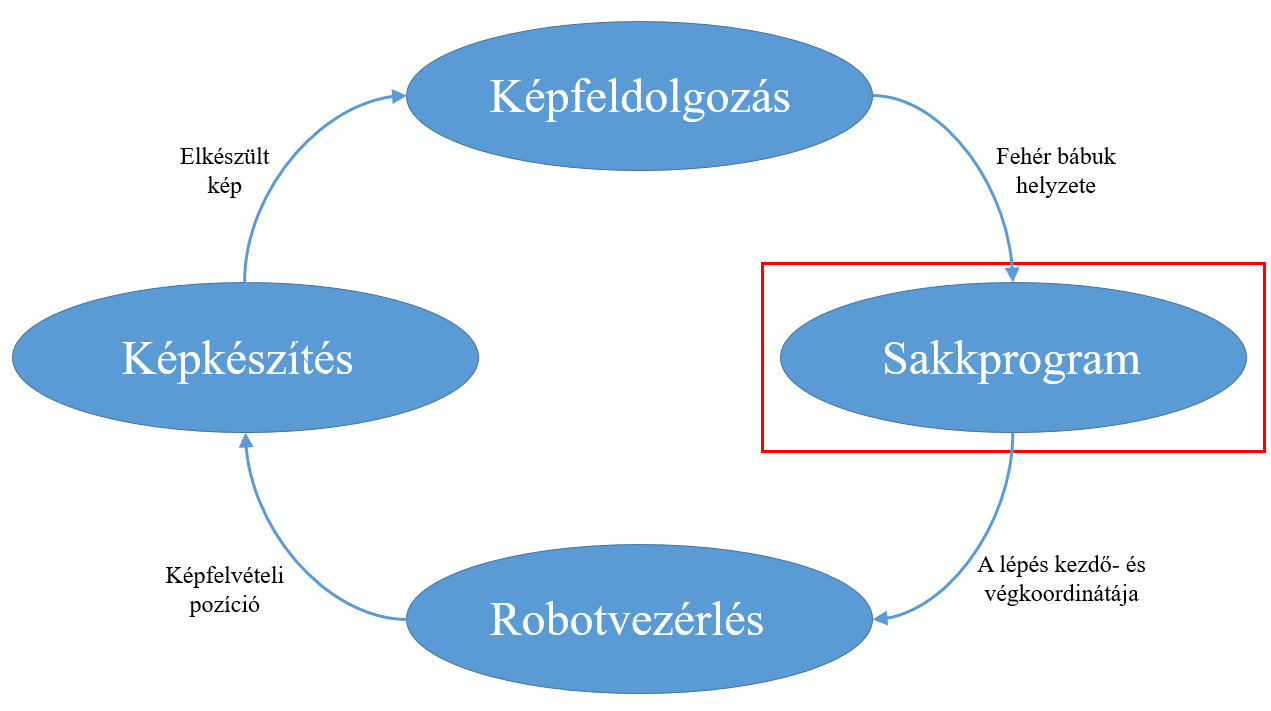
\includegraphics[scale=0.45]{flowchart-chess}
\caption{A sakkprogram helye a folyamatban}
\label{fig:flowchart-chess}
\end{figure}

A képfeldolgozás kimenete egy 8x8-as tömb (mátrix), amely indexelése megegyezik a sakkprogramnál bemutatott mezőindexeléssel (\ref{fig:chessboard} ábra). Ez a tömb az ember lépése utáni állapotban mutatja a bábuk elhelyezkedését. Ahhoz, hogy a megtett lépést meg lehessen határozni, ezt az állapotot össze kell vetni a lépés előttivel. A programben vezetett állást bármikor le lehet kérdezni (sakkjáték példány -> board -> b). A kapott elem egy 8x8-as tömb, amely egyes elemei vagy null értékűek vagy az ott található bábut írják le. Minden bábu esetén le lehet kérdezni, hogy fekete-e vagy fehér (white: bábu \angol{boolean} tulajdonsága - igaz ha fehér, hamis ha fekete). Ezek alapján létre lehet hozni egy olyan logikai értékeket tartalmazó tömbböt, amely formailag megegyezik a képfeldogozó rész által szolgáltatott tömbbel.

A lépés előtti és utáni tömböket a `FindMove' függvény értékeli ki. Elemenként hasonlítja össze a tömböket a program. Ha két elem megegyezik, az azt jelenti, hogy az ott lévő bábu nem mozdult el. Ha különbözik a két érték, akkor két eshetőség állhat fenn:

\begin{itemize}
	\item a bábu ellépett onnan (lépés után `false' a mező értéke) - ekkor ez a mezőkoordináta lesz a lépés kiindulópontja, vagy
	\item a bábu oda lépett (lépés után `true' a mező értéke) - ez a mező a lépés végpontja.
\end{itemize}

Két fehér bábu egy kör alatt csak sánszoláskor mozdulhat el. Ezt az eshetőséget a lépés meghatározásakor külön meg kell vizsgálni. Mivel a fekete bábuk pozícióját a sakkprogram követi, így nem igényel külön eljárás kialakítását az, ha a fehér játékos leüti a fekete egy bábuját. Ilyen esetben a leütőtt bábu pozíciójához a lépés előtt `false' érték tartozott, ezt a sakkprogram adja meg. A képfeldolgozó rész csak a fehér bábukat keresi (azokon van csak zöld jelölő), így az ütés után a mező értéke `true' lesz.

A lépés validálására érdemes meghívni a sakkjáték `checkIfLegalMove' függvényét mielőtt a lépést a programban végrehajtatnánk, mivel szabálytalan lépést is be lehetne vinni.







\end{document}
	%--Eredmények értékelése
	\newpage
	\documentclass[../documentation.tex]{subfiles}
 
\begin{document}
\section{Eredmények, továbbfejlesztési irányok} \label{sec:results}
A projekt 4 főbb modulból áll (képkészítés, képfeldolgozás, sakkprogram és robotvezérlés), ezeket kellett összekötni ahhoz, hogy sakkozásra képessé lehessen tenni a robotkart \aref{sec:projectdescription} fejezetben bemutatott konstrukcióval. A projekt összesített értékelését \aref{sec:osszefoglalas}. fejezet tartalmazza. Ebben a fejezetben az egyes modulok korlátai, kiforrottsága, megbízhatósága és továbbfejleszthetősége kerül taglalásra.

\subsection{Képkészítés értékelése}
A robotvezérlő (KRC4) (és a rajta futó szoftver) kompatibilis a választott Logitech C270 HD webkamerával. A kamerát egyszerűen a robotvezérlőn található USB bemenetek valamelyikére lehet kötni. A robotkar és a robotvezérlő több méteres távolsága miatt USB hosszabító kábelre van szükség, 2 méteres passzív toldókábellel kommunikációs hiba nélkül üzemel a kamera.

A kamera kezelő osztály (CameraHandler.java) HD képes webkamera kezelésére lett kialakítva. Minden bizonnyal egyéb képkészítésre alkalmas eszközt is tudna kezelni, de ez további teszteket igényelne. A kamera megnyitási ideje erősen változó lehet a tipus függvényében: a Logitech kamera esetén ez pár másodperc, míg a Microsoft kameránál fél vagy 1 perc is lehetett. A Windows alapfunkciójaként elérhető kamera alkalmazás mindkettő kamerát 1-2 másodperc alatt megnyitotta, szóval az OpenCV kamerakezelésében lehet különbség.

Továbbfejleszthető ez a modul:
\begin{itemize}
	\item a felbontás és képarány automatikus választásával,
	\item több csatlakoztatott kamera esetén a megfelelő kiválasztásával,
	\item illetve a torzítások ellensúlyozásával.
\end{itemize}

\subsection{Képfeldolgozás megbízhatósága}
A képfeldolgozás alapvetően 2 elemből áll: a mezőkalibrációból és a fehér bábuk kereséséből.

A mezőkalibráció főként a kalibrációs sakktáblamintán található sarokpontok kereséséből áll. Ezek alapján történik a mezőkről (pontosabban a bábuk tetejéről) készült képek kivágása. Az OpenCV 2.4.13.6-os verziónál a 3.4.4 megbízhatóbban működik, ugyanazon a képen megtalál olyan sarokpontokat, amiket a régebbi verzó nem. A sarokpontok megtalálása nem csak a kalibrációs tábláról alkotott képrészlet minőségétól függ, hanem a képen található egyéb mintázatoktól is, főként ha annak vonalai kontrasztosak. A kalibrációs képet utólagosan lehet módosítani, hogy a sakktáblán kívüli részt adott színnel ki legyen töltve. Ezt manuálisan kell megtenni.

A fehér bábuk keresése a mezőkről kapott képeken belüli színszűrésen alapszik. A módszer RGB színskálát használ a zöld színű részek megtalálására, ami átlagosnak mondható fényviszonyok között kifejezetten jól működik. Rosszabb fényviszonyok között nem lett tesztelve a módszer, de ilyen esetben a HSV színskála használata (az RGB helyett) előnyösebb lehet. A tesztelt fényviszonyokkal a képek körülbelül 50\%-át tölti ki zöld szín, ha ott fehér bábu található (a tetejükre zöld lap van ragasztva). Ez alapján a bábuk pozíciójának kiértékelése egyszerű.

Továbbfejleszthetési irányok:
\begin{itemize}
	\item A projekt kidolgozásának idején az OpenCV egy újabb verzióját is kiadták, érdemes lehet azt beépíteni a programba.
	\item A kamerapozíciónálás során a megtalált sarokpontok szinekkel megjelölése (kvázi valós időben) elősegítené a megfelelő pozíció megtalálását, illetve a megfelelő pozíció megtalálását automatizálni is lehetne.
	\item Az \ref{qrsection} fejezetben ismertetett QR kód alapú eljárás kidolgozása további funkciókat tenne elérhetővé.
\end{itemize}

\subsection{A sakkprogram értékelése}
A sakkprogram elsődleges forrása egy kész, Java alapű, felhasználói interfésszel rendelkező program volt, ebből lettek a projekthez szükséges elemek kiemelve. További függvényekkel kellett kiegészíteni ezt a programorészletet ahhoz, hogy a képfeldolgozó és a robotvezérlési modulokkal kompatibilis legyen.

Az sakkprogram magja fel van készítve arra, hogy egy teljes sakkjátszámát le lehessen játszani, viszont a képfeldolgozási résszel összekötés olyan módon lett implementálva, amely a sáncolást nem tudja ilyen formában felismerni és kezelni. Ez a probléma pár függvénykibővítéssel megoldható.

A sakkprogram által használt algoritmus tetszőlegesen módosítható lenne játék közben is, de ennek kezelésére nem készült külön felhasználói bemenet. Jelenleg a sakkprogram kódjának megváltoztatásával lehet ezt állítani.

A program beépített virtuális sakkórát is használ, emellett a játékosok nevei is személyre szabhatóak (ezt a nevet írja ki a program bármely játékoshoz kötődő esemény kiíratásánál). A sakkprogram magja képes lenne adott játékállásból folytatni egy játékot, illetve elmenteni az adott állást.

Ezzel a modullal kapcsolatos legjelentősebb fejlesztési irány a smartPAD-re kidolgozott felhasználói interfész kifejlesztése, így lehetőség nyílna játék közben a különböző paraméterek állítására, illetve a folyamatok monitorozására.

\subsection{A robotvezérlés értékelése}
\subsubsection{A megfogó irányítása}
A robotvezérlő EtherCAT kommunikációt használó, digitális és analóg I/O modulok segítségével tudja vezérelni a megfogót. A jelenleg implementált funkciókhoz elég csak a digitális modulok használata, de az analóg modulokra is szükség van az összes gripperfunkció kihasználáshoz.

A pozícióvisszacsatolás segítene eldönteni, hogy a megfogónak ténylegesen sikerült-e megfognia a bábut. A szorítóerő beállítása jelenleg hardveresen történik, de ezt a programból is lehetne vezérelni.

\subsubsection{A robotkar vezérlése}
A robotkar kalibrálása a sakktáblához gyorsan kivitelezhető. A robot képes a képkészítési pozíció ismételt felvételére, illetve a sakkalgoritmus által meghatározott lépések kivitelezésére, leszámítva azokat a lépéseket, amikhez több bábú mozgatása is szükséges (ütések, sáncolás, en passant). Ezen lépések implementálása nem ütközik hardveres problémába, így viszonylag könnyen megvalósíthatóak.

Továbbfejleszthető elemek:
\begin{itemize}
	\item Ha a robotkar ütközés hatására megáll, akkor jelenleg csak manuálisan lehet visszatéríteni az eredeti program folytatásához. Ezt a visszavezetést a programból is meg lehetne oldani.
	\item A robotkar jelenleg a robot bázis koordinátarendszerben mozog, de praktikusabb lenne a sakktáblához rendelt bázist használni. Ekkor a folyamatok a sakktábla különböző irányú dőléseire sokkal kevésbé lennének érzékenyek.
	\item A sakktábla bázispontjának felvétele ``handguiding'' (kézi vezetés) használatával gyorsabb és kényelmesebb lenne.
\end{itemize}






















\end{document}
%---------------------------------------------------------

%--Összefoglalás------------------------------------------
%\include{sections/summary}
%---------------------------------------------------------

%--Források-----------------------------------------------
%\addcontentsline{toc}{section}{Források}
% \bibliographystyle{unsrt}
%\bibliographystyle{acm}
%\bibliography{bibdata}
%---------------------------------------------------------

%--Angol összefoglalás------------------------------------
%\include{sections/summary_en}
%---------------------------------------------------------

\end{document}